\subsection{Dynamics results}
\label{subsec:molecular_dynamics_results}

First we look into relaxation of the order parameter to the equilibrium values. For that we perform Langevin Dynamics simulation for a set of simulation parameters as described in \ref{subsec:simulation_details}.




We start by looking into system evolution on a short time scale. For that we analyse time dependence of the order parameter~\eqref{eq:nematic_order_parameter} starting from different initial configurations outlined in previous section. The results for different densities are presented on the Figure~\ref{fig:short_time_order_parameter_different_density}. The squares stands for random initial configuration, the circles for co-aligned and triangles for counter-aligned initial configuration.

\begin{figure}[h]
\centering
\begin{subfigure}[t]{0.32\textwidth}
	\centering
	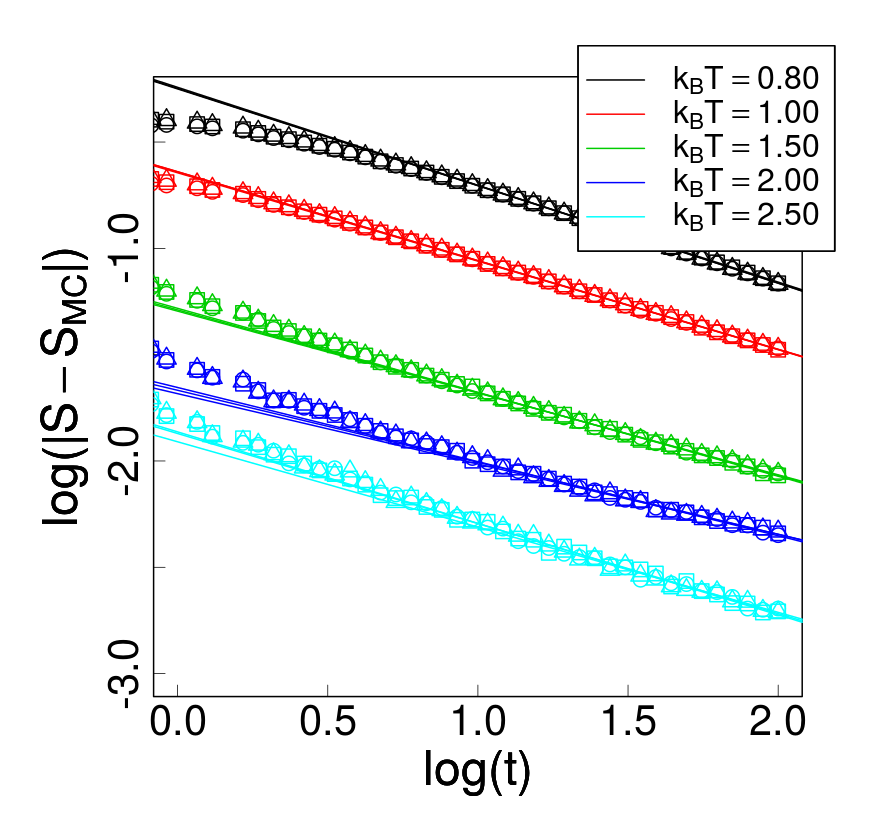
\includegraphics[width=\textwidth]{Images/relax_25.png}
	\captionsetup{justification=centering, width=0.9\columnwidth}
	\caption{$\rho = 0.25$}
\end{subfigure}
\begin{subfigure}[t]{0.32\textwidth}
	\centering
	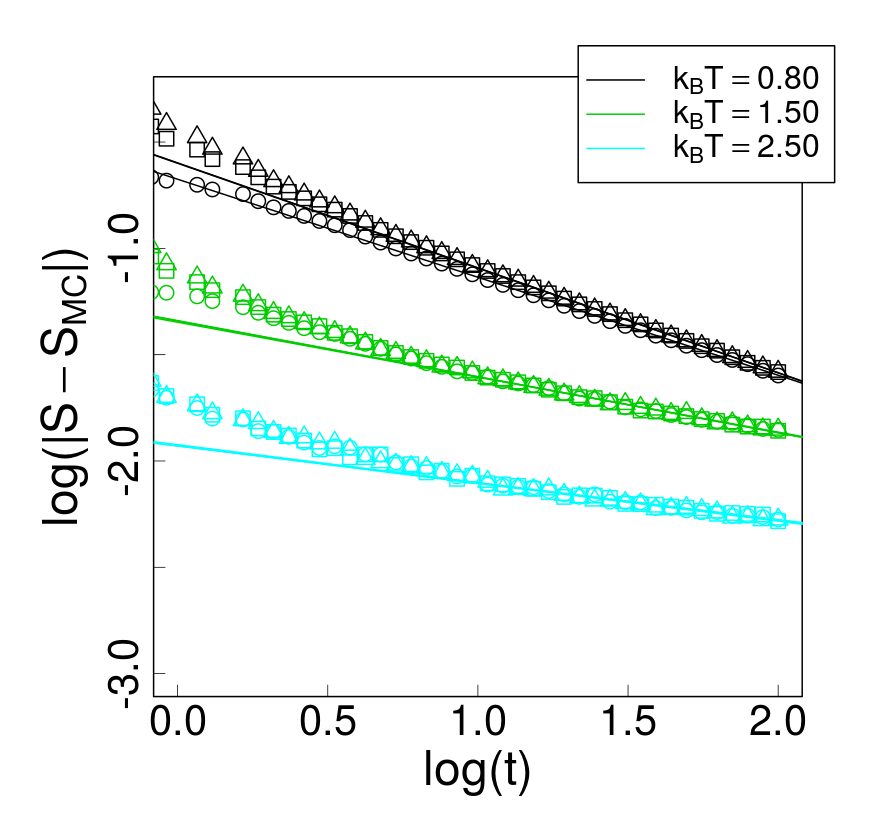
\includegraphics[width=\textwidth]{Images/relax_50.png}
	\captionsetup{justification=centering, width=0.9\columnwidth}
	\caption{$\rho = 0.5$}
\end{subfigure}
\begin{subfigure}[t]{0.32\textwidth}
	\centering
	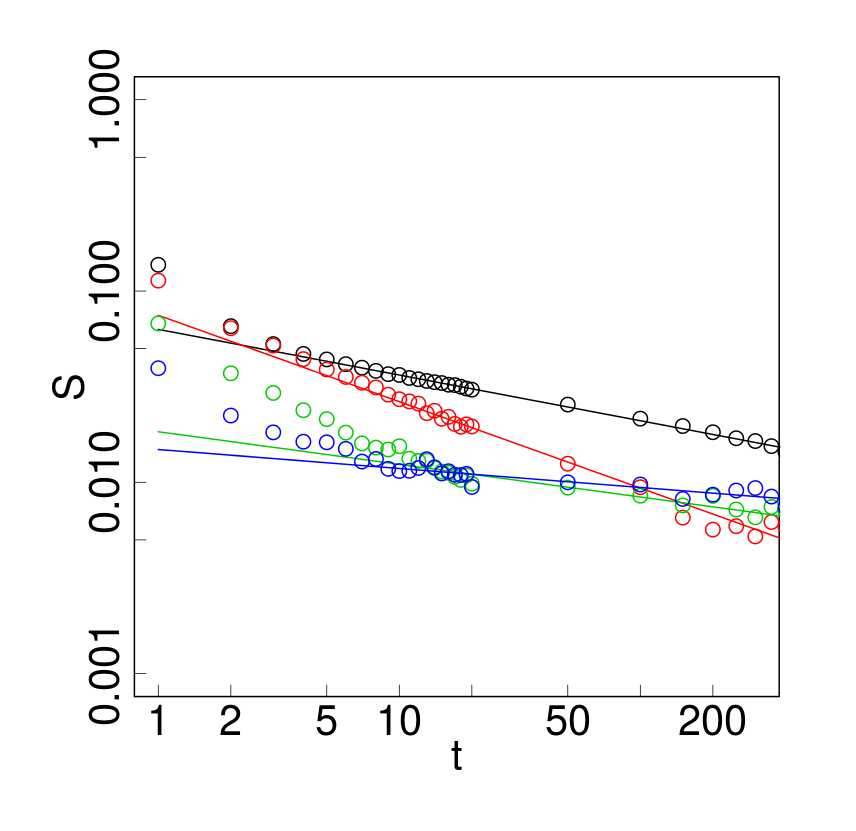
\includegraphics[width=\textwidth]{Images/relax_75.png}
	\captionsetup{justification=centering, width=0.9\columnwidth}
	\caption{$\rho = 0.75$}
\end{subfigure}
\captionsetup{justification=centering, width=0.9\columnwidth}
\caption{Order parameter as function of simulation time for different $k_BT$ and $\rho$. Squares indicates random initial configuration, circles --- co-aligned, and triangles --- counter-aligned. The simulations are performed for $N = 1600$ particles and the results are averaged over $100$ samples}
\label{fig:short_time_order_parameter_different_density}
\end{figure}
